

%Tähän voisi laittaa kuvan komponenttien asemmoitumisesta toisiinsa.
\subsubsection{Asiakaslaite}
Asiakaslaite (user equipment) on yleisnimitys reunan tai pilven palveluita kuluttavalla laitteelle.
Asiakaslaite -käsitettä ei ole rajattu mihinkään tiettyihin laitteisiin ja asiakaslaite voikin olla esimerkiksi älypuhelin, älylasit tai verkkoyhteydellä varustettu auto. 
Asiakaslaitteiden yhdistävänä tekijänä on siis jonkinlainen yhteys reuna- tai pilvipalveluihin. Yleisesti asiakaslaitteen käyttämä yhteys on tyypiltään langaton. 
Yksinkertaisuuden vuoksi tässä tutkielmassa asiakaslaitteen voi ajatella älypuhelimena, jollei toisin mainita.

Verkkohierarkian näkökulmasta asiakaslaitteet ovat lehtisolmuja. Tämä tarkoittaa että asiakaslaitteet toimivat ainoastaan palveluiden kuluttajina eivätkä siis tarjoa itse palveluita. Myöskään kulutettavien palveluiden tyypillä ei ole juurikaan merkitystä, kun asiaa käsitellään infrastruktuuri tai arkkitehtuuritasolla.

Konkreettinen esimerkki asiakaslaitteesta, joka hyödyntää reunapalvelua, voisi olla jokin ajoneuvo.
Ajoneuvolla on mobiiliyhteys reunapalveluun jonka tarkoitus on välittää tietoa liikenteestä muille ajoneuvoille. Esimerkiksi tilanteessa jossa edellä on ruuhkaa, voitaisiin muille lähistöllä oleville ajoneuvoille välittää tieto tästä, jolloin voidaan valita jokin toinen reitti määränpäähän.

%Asiakaslaite on yleisnimitys laitteelle, joka hyödyntää reunan tai pilven tarjoamia palveluita jonkin tietoliikenneyhteyden avulla.
%Reunalaskentaa käsittelevässä kirjallisuudessa asikaslaitteeseen viitataan usein UE (User Equipment) termillä. 
%Se mitä konkreettista laitetta asiakaslaitteella tarkoitetaan riippuu kontekstista. 
%Tässä tutkielmassa asiakaslaitteella tarkoitetaan älypuhelinta jollei toisin mainita. 
%Esimerkkinä jostain toisesta asiakaslaitteesta on auto, joka on varustettu mobiiliverkkoyhteydellä. Auto voi käyttää reunapalveluita esimerkiksi kommunikoidakseen muiden lähistöllä olevien autojen kanssa.
%Asiakaslaitteet verkkoyhteyksien muodostaman hierarkian "lehtisolmuja" joka tarkoittaa että ne eivät enää tarjoa palveluitaan muille asiakaslaitteille. 


\subsubsection{Reuna} \label{reunatoimijat}
Reuna koostuu useista toiminnallisista entiteeteistä, jotka voidaan jakaa sekä fyysisiin, että loogiisin kokonaisuuksiin. 
Tässä kappaleessa lähdemme liikkeelle määrittelemällä reuna-alueen, joka edustaa reunan toimialuetta, sekä reunaa yleisenä käsitteenä.
Tämän jälkeen esitellään reunasolmu, joka on reunajärjestelmän keskeisin fyysinen rakennuspalanen. Lopuksi esitellään pääasiassa ohjelmallisen tason toimivat toimijat reuna-alusta ja reunasovellus.

\paragraph{Reuna-alue} 
Yleisesti puhuttaessa reunalla viitataan alueeseen, joka ulottuu asiakaslaitteelta runkoverkkoon asti. Reuna-alue siis alkaa asiakaslaitteelta ja laajenee kohti internettiä.
Reunalla ei siis ole tarkkaa määritelmää, vaan termiä usein sovelletaan käytettävän kontekstin mukaan siten, että reuna-alue rajautuu kontekstissa esiintyvien toimijoiden mukaan edellä manitulle välille.
Esimerkiksi mobiiliverkon tukiasemien yhteyteen rakennettua reunajärjestelmää käsiteltäessä, reunalla tarkoitetaan ainoastaan reunajärjestelmän asiakaslaitteita palvelevien osien muodostamaa vyöhykettä. 
Kuten jo aiemmin mainittu, reunan keskeisenä etuna muihin palveluihin voidaan pitää reunapalveluiden ja asiakaslaitteen välisen viiveen vähäisyyttä.
Yleisenä nyrkkisääntönä reunalle voidaankin pitää verkkoyhteyksien viivettä suhteessa muuhun internettiin, koska reuna-alueella viiveiden tulisi siis olla muuta internettiä nopeampia. Toisin sanoen reunan palveluiden tulisi sijaita lähempänä kuin pilvessä sijaitsevien palveluiden.


\paragraph{Reunasolmu} 
Tämän tutkielman kontekstissa reunasolmulla (mobile edge host) tarkoitetaan yksittäistä reunalaskentaa tarjoavaa entiteettiä\cite{etsirefarch}.
Reunasolmu -termillä viitaataan reunasolmun fyysiseen laitteiston ja reunasolmun toiminnalliseen kokonaisuuteen.
Reunasolmu sisältää reunasovelluksien suorittamiseen tarvittavat resurssit, joita ovat laskenta, tallennustila ja verkkoyhteydet.
Reunasolmu voi koostua esimerkiksi mobiilitukiaseman ja palvelinlaitteiston muodostamasta kokonaisuudesta. 
Reunasolmun toiminnallinen kokonaisuus sisältää erinäisiä toimintoja, joiden tehtävänä on mahdollistaa reunasovelluksien suorittaminen. Tällaisia ovat muun muassa tietoliikenteen reitittäminen ja virtualisointi-alustan tarjoaminen, sekä sen hallinnointi. Myös seuraavassa kappaleessa käsiteltävä reuna-alusta kattaa osan reunasolmun toiminnoista.

Kuten aiemmin mainittu, reunajärjestelmä koostuu joukosta reunasolmuja, jotka ovat maantieteellisesti hajautettuja.
Reunasolmut siis eroavat toisistaan vähintään sijainnin perusteella, mutta voivat erota myös käytettävissä olevien resurssien osalta. Resurssien osalta reunasolmu voi olla mitä tahansa vähäisillä laskenta ja tallennus resursseilla varustetun WiFi-tukiaseman ja kokonaisen palvelinklusterin väliltä.
Reunasolmun sijaintiin vaikuttaa käytössä oleva reuna-arkkitehtuuri.
%Kuten juuri mainittu, reunasolmujen sijaintiin vaikuttaa käytettävä reuna-arkkitehtuuri.
Reunan rakennetta ja  reunasolmujen sijaintia käsitellään tarkemmin luvussa \ref{rakenne}.

\paragraph{Reuna-alusta}
Reuna-alusta (Edge platform) on ohjelmistotason toimija. Se tarjoaa rajapinnan reunasovelluksien suorittamista varten. Toisin sanoen se siis tarjoaa reunasovelluksille toimintaympäristön.
Reuna-alustan tehtävät eivät rajaudu ainoastaan yksittäiseen reunasolmuun, vaan sen lisäksi se hoitaa hallinnollisia tehtäviä kuten tietoliikenteen ohjausta. Lisäksi reuna-alustan tehtäviin voidaan lukea reunasovelluksia suorittaviin virtuaalikoneisiin liittyvät hallinnolliset toimet. Esimerkkinä reuna-alustan tehtävistä on kappaleessa \ref{livemigraatio} esiteltävä virtuaalikoneiden live migraatio reunasolmulta toiselle.
Reunasovelluksien lisäksi reuna-alusta voi itsessään tarjota palveluita, jotka eivät suoranaisesti ole reunasovelluksia vaan esimerkiksi nopea kommunikaatioväylä laitteelta-laitteelle (machine-to-machine), jota voi käyttää vaikka ajoneuvojen väliseen viestintään.

\paragraph{Reunasovellus}
Reunasovelluksella (Edge application) tarkoitetaan yksittäistä reunasolmulla suoritettava ohjelmistoa, jonka kuluttajana voi toimia asiakaslaite tai toinen reunasovellus. Reunasovellus ei ota kantaa millaista palvelua sillä tuotetaan ja sen rajoitteet asettaa pääasiassa käytössä oleva reuna-alusta. 

Reunasovelluksen tuottama palvelu voi olla tyypiltään yhteiskäyttöinen tai käyttäjäkohtainen, esimerkiksi käyttäjäkohtainen virtuaalikone johon käyttäjä voi ottaa etäyhteyden. Esimerkki yhteiskäyttöisestä reunasovelluksesta olisi pelipalvelin, jota voivat käyttää reunasolmun lähistöllä olevat pelaajat. 

\subsubsection{Pilvi}
%kirjoita uusiksi
Pilvellä tarkoitetaan internetin ytimen läheisyydessä sijaitsevaa aluetta.
Pilven voidaan ajatella laajenevan kohti reunaa. Koska pilven ja reunan raja ei ole selkeä ne voivat olla limittäin.
Tavallisessa asiakas-palvelin -mallissa palvelun tuottavan palvelimen voidaan ajatella sijaitsevan pilvessä. Kun mukaan otetaan reunajärjestelmä, palveluiden tuottaminen hajautuu reunan ja pilven kesken. Reunanjärjestelmän ei ole tarkoitus korvata pilveä vaan täydentää sitä. 


%Asiakaskohtaiselle reunainstanssille ei ole mitään vakiintunutta nimeä.
%Cloudlet on yksi ehdotettu toteutustekniikka tällaiselle asiakaskohtaiselle reunalla sijaitsevalle virtuaali-instanssille \cite{satya09}.

\subsubsection{Mobiiliverkko}
\begin{figure}[tb]
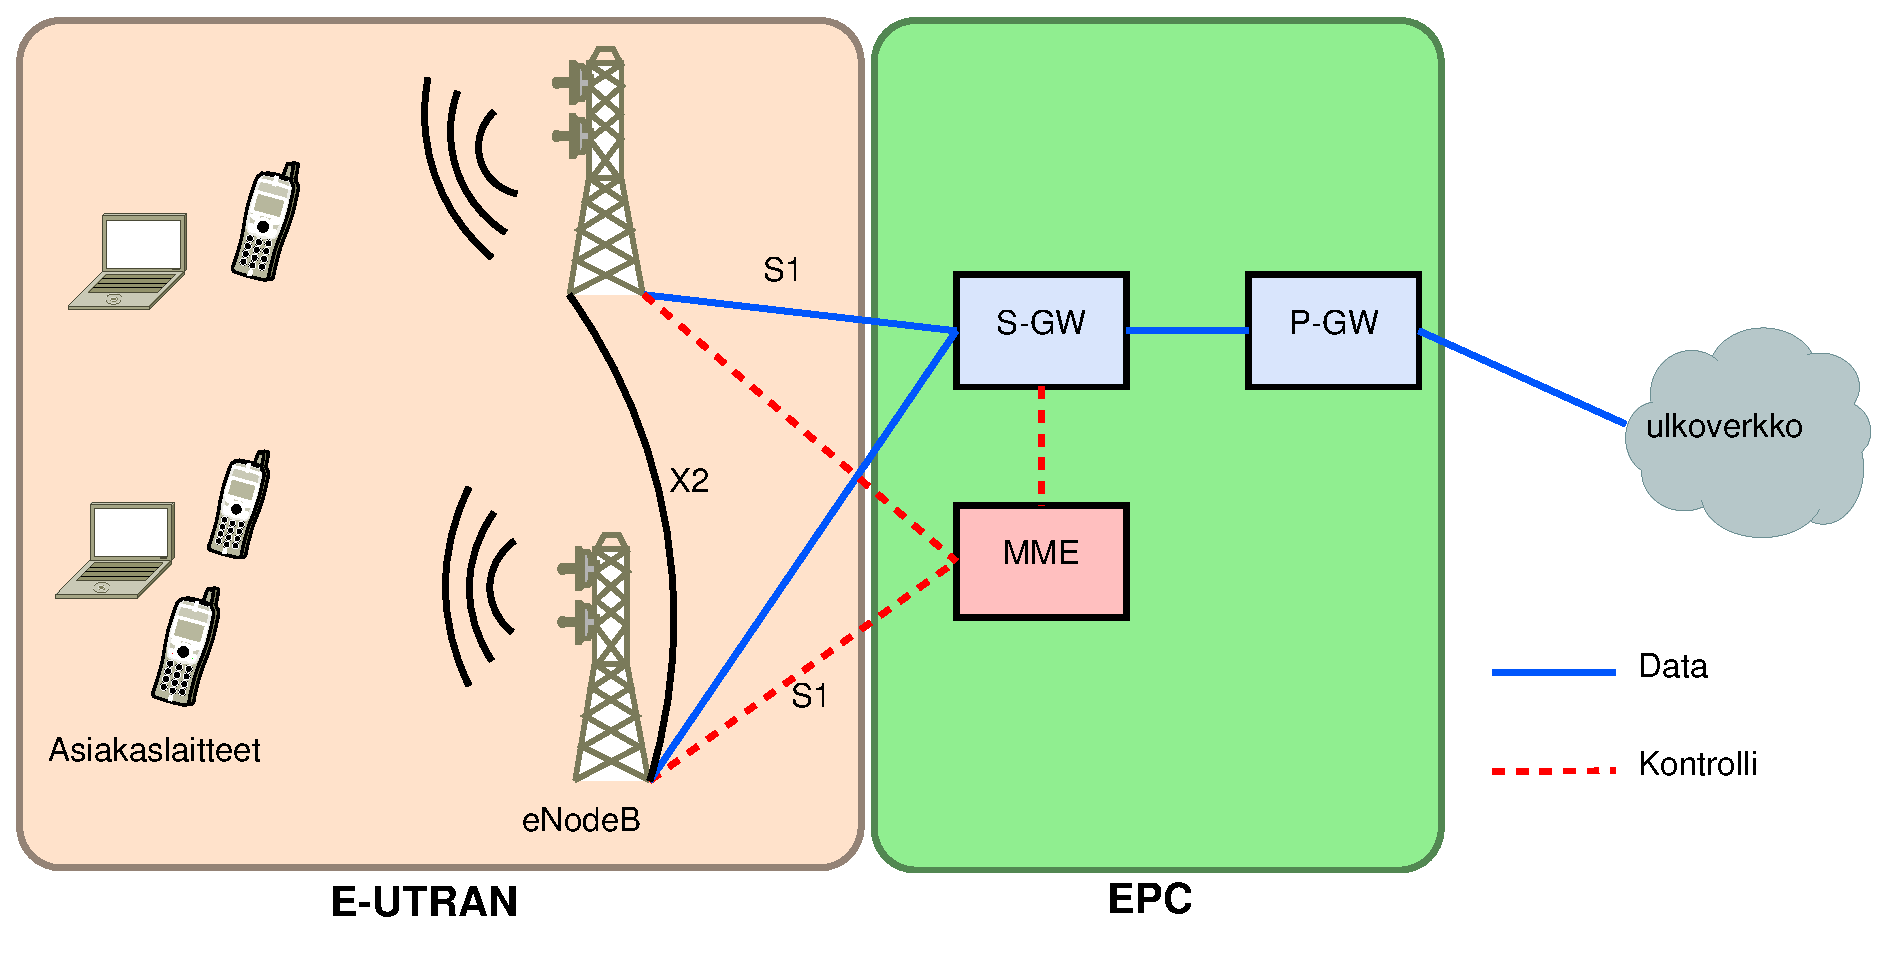
\includegraphics[width = \textwidth]{EPC.eps}
\caption{Yksinkertaistettu LTE-tyyppisen mobiiliverkon rakenne.} \label{fig:mobiarch}
\end{figure}

Tässä tutkielmassa käsiteltävät reuna-arkkitehtuurit sisältävät yhdistävänä tekijänä tavoitteen toimia mobiiliverkon yhteydessä. 
Täten reuna-arkkitehtuurien suunnittelupäätöksiä tarkasteltaessa on tarpeen ymmärtää mobiiliverkon osat yleisellä tasolla.
Yksinkertaisuuden vuoksi tämän tutkielman puitteissa mobiiliverkoksi oletetaan LTE:n mukainen arkkitehtuuri, joka koostuu E-UTRAN tyyppisestä radioverkosta ja EPC tyyppisestä runkoverkosta.
Seuraavaksi käydään läpi mobiiliverkon arkkitehtuurin tämän tutkielman kannalta merkitykselliset toimijat ja toiminnot.

Korkealla tasolla tarkasteltuna mobiiliverkko koostuu kahdesta osiosta: radioverkosta ja runkoverkosta. 3GPP kehittämässä LTE (Long Term Evolution) standardissa radioverkon sisältävä osuus on nimeltään E-UTRAN (Evolved UMTS Terrestrial Radio Access Network) ja runkoverkon osuus on nimeltään EPC (Evolved Packet Core).
E-UTRAN ja EPC väliset yhteydet on kuvattu kuvassa \ref{fig:mobiarch}.

E-UTRAN tehtävänä on toimia rajapintana asiakaslaitteen ja EPC:n välillä. 
E-UTRAN sisältää verkon puolella pääasiallisena toimijana eNodeB (Evolved nodeB) tyyppisiä tukiasemia \cite{etsieutran}.
Tukiasemista on olemassa muutamia erilaisia variaatioita, mutta tässä tutkielmassa käsitellään ainoastaan perustapausta.
Tukiasema on asiakaslaitetta lähimpänä sijaitseva funktionaalinen verkon osa ja sen seurauksena se on houkutteleva kohde reunalaskennan ratkaisuille. Tietoliikenteen näkökulmasta tukiaseman voi ajatella \textit{reunan} viimeisenä etappina ennen asiakaslaitteita. 

ENodeB tarjoaa asiakaslaitteiden suuntaan radioyhteyden.
EPC:n suuntaan eNodeB:t ovat yhteydessä S1 rajapinnan avulla.
Lisäksi eNodeB:t voivat olla toisiinsa yhteydessä X2 rajapinnan kautta.
S1:stä käytetään eNodeB:n ja EPC:n väliseen kommunikointiin. Tämä sisältää sekä hallinnollisen viestinnän, että asiakkaan tietoliikenteen kuljettamisen.
X2 rajapintaa puolestaan käytetään tukiasemien väliseen kommunikointiin. 
ENodeB välisten X2 yhteyksien tavoitteena on nopeuttaa tukiasemien välistä kommunikaatiota, esimerkiksi handoverin yhteydessä tehtävää asiakaskontekstin siirtoa varten \cite{3gpplte}.
Handoverilla tarkoitetaan asiakaslaitteen radioyhteyden siirtoa toiselle tukiasemalle. Handover käsitellään tarkemmin kappaleessa \ref{livemigraatio}.

Mobiiliverkon runkona toimiva EPC koostuu useista loogisista komponenteista.
Tämä siis tarkoittaa että toiminnallisuudet voivat fyysisesti sijaita samassa laitteessa. 
Tässä tutkielmassa on tarpeen ymmärtää perusteet seuraavista alikomponentista: MME (Mobility Management Entity), S-GW (Serving Gateway) ja PDN GW (P-GW, Packet data network gateway) \cite{etsilte}.
\begin{itemize}
\item \textbf{MME} on EPC:n hallinnollinen entiteetti joka vastaa muun muassa asiakaslaitteen tunnistamisesta ja handoveriin liittyvistä toimista EPC:n sisällä. Toisin kuin S-GW ja P-GW, MME ei käsittele asiakaslaitteiden tietoliikennettä.
\item \textbf{S-GW} eli palveluyhdyskäytävä toimii asiakaslaitteen EPC:n sisäisenä kiintopisteenä.  S-GW reitittää asiakaslaitteen liikennettä P-GW:n ja E-UTRAN välillä.
\item \textbf{P-GW} eli pakettiverkon yhdyskäytävän tehtävänä on toimia asiakaslaitteen ja mobiiliverkon ulkopuolisten IP-verkkojen yhteyspisteenä.
\end{itemize}
\cite{3gppepc}

Mobiiliverkossa käytävä kommunikaatio voidaan jakaa kahteen kerrokseen: kontrollikerrokseen ja tietoliikennekerrokseen.
Kontrollikerroksella välitettävät viestit ovat tarkoitettu hallinnollisiin toimintoihin mobiiliverkon sisällä. 
Tietoliikennekerros välittää asiakkaan tietoliikennettä internetin ja asiakaslaitteen välillä.
Asiakkaan tietoliikenne kulkee tukiaseman ja P-GW:n välillä GTP-tunneloituna (GPRS Tunnelling Protocol) \cite{puente15seamless}. Tämä tarkoittaa että mobiiliverkon sisällä tietoliikennettä ei ohjata asiakaslaitteen tietoliikenteen tunnisteiden pohjalta. 


\subsection{Reuna-arkkitehtuuri}
%Määrittele mikä on reuna-arkkitehtuuri


Tässä tutkielmassa käsiteltävät arkkitehtuurit ovat pääasiassa tyypiltään oletusarkkitehtuureja (framework). 
Tämänkaltaisen arkkitehturin tarkoituksena on jakaa järjestelmä toiminnallisiin osiin fyysisellä ja ohjelmallisella tasolla \cite{ohark}. Se siis kuvaa järjestelmän rakenneosien tehtävät.
Oletusarkkitehtuuria voidaan hyödyntää varsinaista toteutettavaa järjestelmää suunniteltaessa.

Kappaleessa \ref{reunatoimijat} kuvattujen reunan toimijoiden osalta reuna-arkkitehtuurit keskittyvät kuvaamaan reunasolmun ja reuna-alustan tehtäviä. Lisäksi reuna-arkkitehtuurit kuvaavat koko järjestelmän osana toista järjestelmää, jolloin reunajärjestelmä itsessään on komponentti suuremmassa järjestelmässä. Tällä tasolla tarkasteltu arkkitehtuuri jättää avoimeksi reunasovelluksien toiminnan ja keskittyy kuvaamaan reunasovelluksien sijaintia järjestelmässä.

Tämän tutkielman puitteissa arkkitehtuurilla tarkoitetaan reuna-alustan ja reunasolmujen muodostamaa järjestelmää. Reuna-alustan toiminnallisuuksia voisi eritellä vielä tarkemmin, etenkin reunasovelluksien hallinnan osalta. Cloudlet on konkreettinen toteutus reuna-alustan reunasovelluksia hallinnoivasta osasta, mutta se ei kata kuin yhden reunasolmun kerrallaan. 
Tämän lisäksi olemassa on reunasolmujen välisestä hallinnasta vastaava kerros, tosin tämä kerros voi olla ulkoistettu erillisille hallinnolliselle toimijalle, jolloin hallinnollinen osa reuna-alustasta on varsinaisten reunasolmujen ulkopuolella. 

Reunasovelluksien toimintaa ei käsitellä tarkemmin. Taxonomy paperissa on hyvä jaottelu erilaisista sovelluksista. Tämä aihepiiri laajenee sovelluksien jakamiseen osittain reunalla suoritettaviin (offloading) tai mobiilisovelluksen suoritusta tukeviin sovelluksiin. 

